\section{Evaluation} \label{sec:evaluation}

\subsection{Dataset}

For testing the transcription system, we employ the Bach10 dataset \cite{Duan2010}, which is a freely available multi-track collection of multiple-instrument polyphonic music. It consists of ten recordings of J.S. Bach chorales, performed by violin, clarinet, saxophone, and bassoon. Pitch ground truth for each instrument is also provided. Due to the tonal and homogeneous content of the dataset, it is suitable for testing the incorporation of music language models in a transcription system. For training the transcription system, pre-extracted and pre-shifted spectral templates are extracted for the instruments present in the dataset, using isolated note samples from the RWC database \cite{Goto2003}. 

For training the MLMs we use the Nottingham dataset\footnote{ifdo.ca/$\sim$seymour/nottingham/nottingham.html}, a collection of 1200 music pieces in symbolic ABC format, which contain simple chord combinations and tunes. We trained the RNN and the RNN-NADE models using both Stochastic Gradient Descent (SGD) and HF to compare performance. The inputs to both the models are sequences of length 200 where each frame of the sequence is a binary vector of length 88 which covers the full piano note range. We train both the RNN and the RNN-NADE to predict the next vector given a sequence of input vectors. We train the models by minimizing the negative log-likelihood of the sequences using the cross-entropy $ \sum_{i}t_{i}\log p_{i} + (1 - t_{i})\log(1-p_{i})$ where $i$ sums over all the dimensions of the binary vector and $t_i$ is the pitch target.


\subsection{Metrics}


For evaluating the performance of the proposed system for multi-pitch detection, we employ the precision ($\mathit{Pre}$), recall ($\mathit{Rec}$), and F-measure ($\mathit{F}$) metrics, which are commonly used in transcription evaluations \cite{MIREX}.
%\begin{equation}
% \mathit{Pre} = \frac{N_{\mathit{tp}}}{N_{\mathit{sys}}},\ \
%\ \mathit{Rec} = \frac{N_{\mathit{tp}}}{N_{\mathit{ref}}},\
%\ \ \mathit{F} = \frac{2\cdot\mathit{Rec}\cdot\mathit{Pre}}{\mathit{Rec}+\mathit{Pre}}
%\label{eq:PRF}
%\end{equation}
%where $N_{\mathit{tp}}$ is the number of correctly detected pitches, $N_{\mathit{sys}}$ is the number of detected pitches, and $N_{\mathit{ref}}$ is the number of ground-truth pitches. 
As in the public evaluations on multi-pitch detection carried out through the MIREX framework \cite{MIREX}, a detected note is considered correct is if its pitch is the same as the ground truth pitch and its onset is within a 50ms tolerance interval of the ground-truth onset.

\subsection{Results}

To validate the performance of the MLMs, we calculate the prediction precision on unseen sequences of music from the Nottingham dataset. The Nottingham dataset contains 1200 folk melodies out of which we utilise 694 tracks for training, 173 tracks for validation and 170 for testing \footnote{http://www-etud.iro.umontreal.ca/~boulanni/icml2012}. For both the RNN and RNN-NADE models we sample 10 vectors from the conditional distribution at each time-step and calculate the expected precision against the ground truth. The reported precision is found by finding the mean over the predictions of every frame. Table \ref{tab:prediction} shows the results of the validation experiments. These results are of the same order as the prediction accuracies reported in \cite{Boulanger-Lewandowski2012}. We found that for both the models, HF optimization gave better precision than SGD. Training with HF was also easier as there were less hyper parameters to be tuned when compared 
to SGD where learning rate needs to be updated to make sure training is effective. 

\begin{table}[t]
 \begin{center}
 \resizebox{150pt}{!}{
 \begin{tabular}{|l|c|}
  \hline
  \textbf{Model} & $\mathit{Pre}$ \\ \hline 
  RNN (SGD)  & 67.89\% \\ \hline
  RNN (HF) & 69.61\% \\ \hline
  RNN-NADE (SGD) & 68.89\% \\ \hline
  RNN-NADE (HF)  & \textbf{70.61}\% \\ \hline
     
 \end{tabular}
 }
\end{center}
 \caption{Validation results for MLMs}
 \label{tab:prediction}
\end{table}


Multi-pitch detection experiments are performed using the proposed system, with various configurations. A first configuration only considers the transcription system from Section \ref{sec:transcription}. A second configuration takes the output of the transcription system and gives it as input to the prediction system of Section \ref{sec:prediction}, where the final piano-roll is the output of the prediction step. A third configuration (presented in Section \ref{sec:combination}), re-transcribes the recording, having the prediction as a prior information for estimating the pitch activations. For the prediction system, experiments were made using both the RNN-NADE and the RNN.

Results using the various system configurations are displayed in Table \ref{tab:results}. It can be seen that the best performance is achieved by the 3rd configuration when using the NADE-HF model for prediction, which surpasses the acoustic-only transcription system by more than 3\%. In general, it can be seen that by using the prediction system as a post-processing step (2nd configuration) always leads to an improvement over the acoustic-only model (1st configuration). A similar trend can be observed when integrating the prediction information as a prior in the transcription system (configuration 3) compared to just using the prediction system as post-processing (configuration 2); an improvement is always reported. Another observation can be made when comparing the RNN-NADE with the RNN, with the former providing a clear improvement. 

Qualitatively, the MLMs are able to improve transcription performance by providing a rough estimate of which pitches are expected to appear in the recording (and which pitches are not experted to appear). The language models were trained using simple chord sequences (from the Nottingham dataset) that are representative of simple tonal music and are applicable as language models to the more complex Bach chorales.

As an example of the proposed system's performance, the spectrogram and raw output of the transcription-prediction system using the 3rd configuration is displayed for a recording from the Bach10 dataset in Fig. \ref{fig:Spectrogram}, whereas the post-processed transcription output along with the ground truth for the same recording is shown in Fig. \ref{fig:Transcription}.

For comparison with the method of \cite{Duan2010} (where the Bach10 dataset was first introduced), the proposed method using the frame-based accuracy metric which is defined in the same paper by Duan et al., reaches 74.3\% for the NADE-HF using the 3rd configuration, whereas the method of \cite{Duan2010} reaches 69.7\% (with unknown polyphony).

\begin{table}[t]
 \begin{center}
 \resizebox{230pt}{!}{
 \begin{tabular}{|l|c|c|c|}
  \hline
  \textbf{Configuration} & $\mathit{F}$ & $\mathit{Pre}$ & $\mathit{Rec}$  \\ \hline 
  Configuration 1 & 62.02\%  & 58.51\% & 66.12\% \\ \hline
  Configuration 2 - NADE & 62.62\% & 59.70\% & 65.92\% \\ \hline
  Configuration 3 - NADE & 64.08\% & 61.96\% & 66.44\% \\ \hline
  Configuration 2 - RNN & 62.29\% & 59.08\% & 65.98\% \\ \hline
  Configuration 3 - RNN & 63.85\% & 61.14\% & 66.90\% \\ \hline  
  Configuration 2 - NADE-HF & 62.20\% & 59.14\% & 65.68\% \\ \hline
  Configuration 3 - NADE-HF & \textbf{65.16}\% & \textbf{62.80}\% & \textbf{67.78}\% \\ \hline  
  Configuration 2 - RNN-HF & 62.44\% & 59.28\% & 66.07\% \\ \hline
  Configuration 3 - RNN-HF & 62.87\% & 60.03\% & 66.11\% \\ \hline    
 \end{tabular}
 }
\end{center}
 \caption{Transcription results using various system configurations.}
 \label{tab:results}
\end{table}


\begin{figure}[t]
 \resizebox{230pt}{!}{
 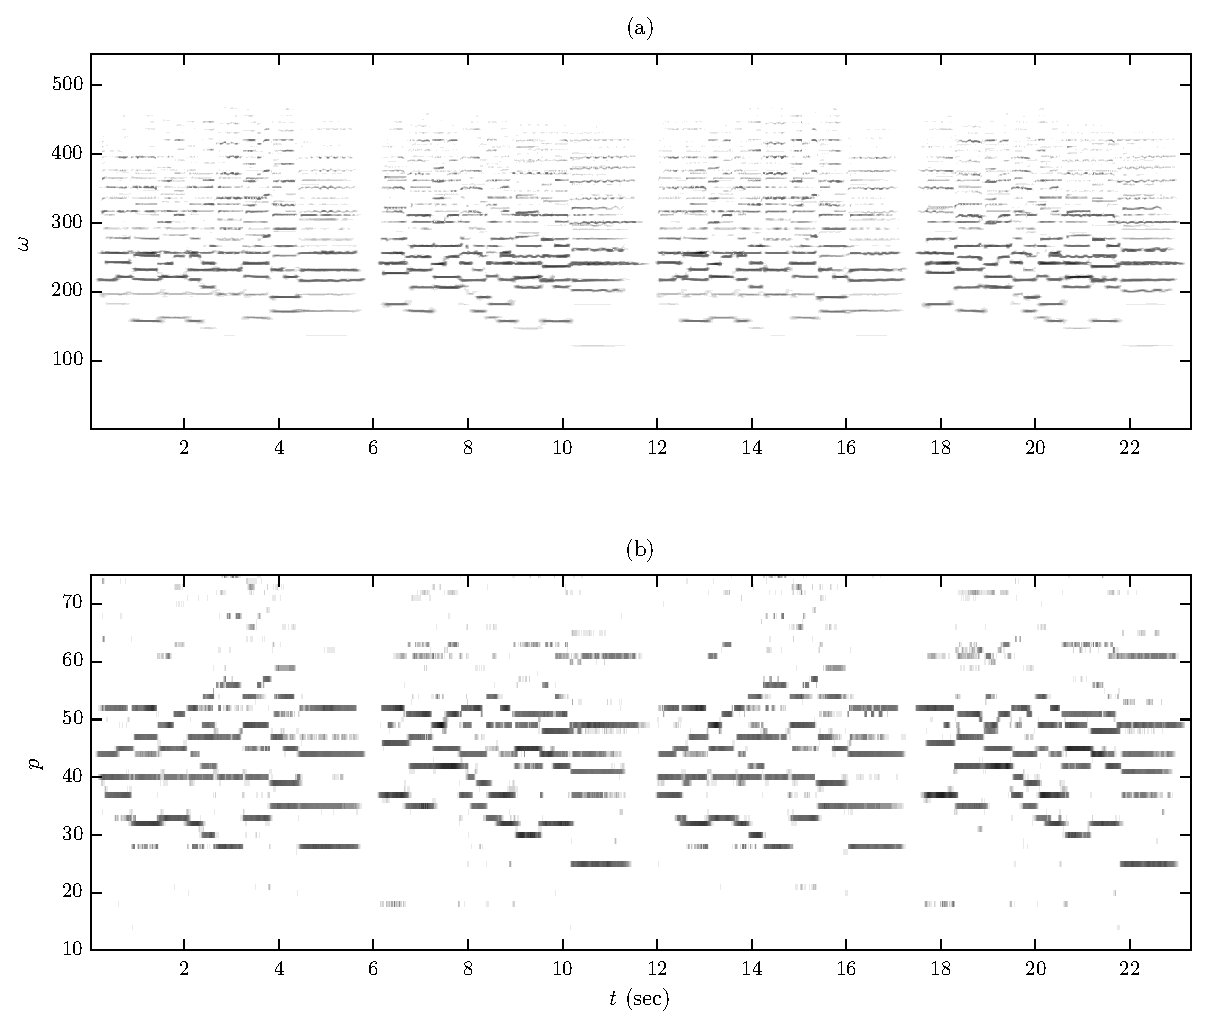
\includegraphics{figures/FigSpectrogram.eps}
 }
 \caption{(a) The spectrogram $V_{\omega,t}$ for recording ``Ach Lieben Christen'' from the Bach10 dataset. (b) The pitch activation $P(p,t)$ using the  transcription-prediction system using the 3rd configuration, with the NADE-HF.}
 \label{fig:Spectrogram}
\end{figure}

\begin{figure}[t]
 \resizebox{230pt}{!}{
 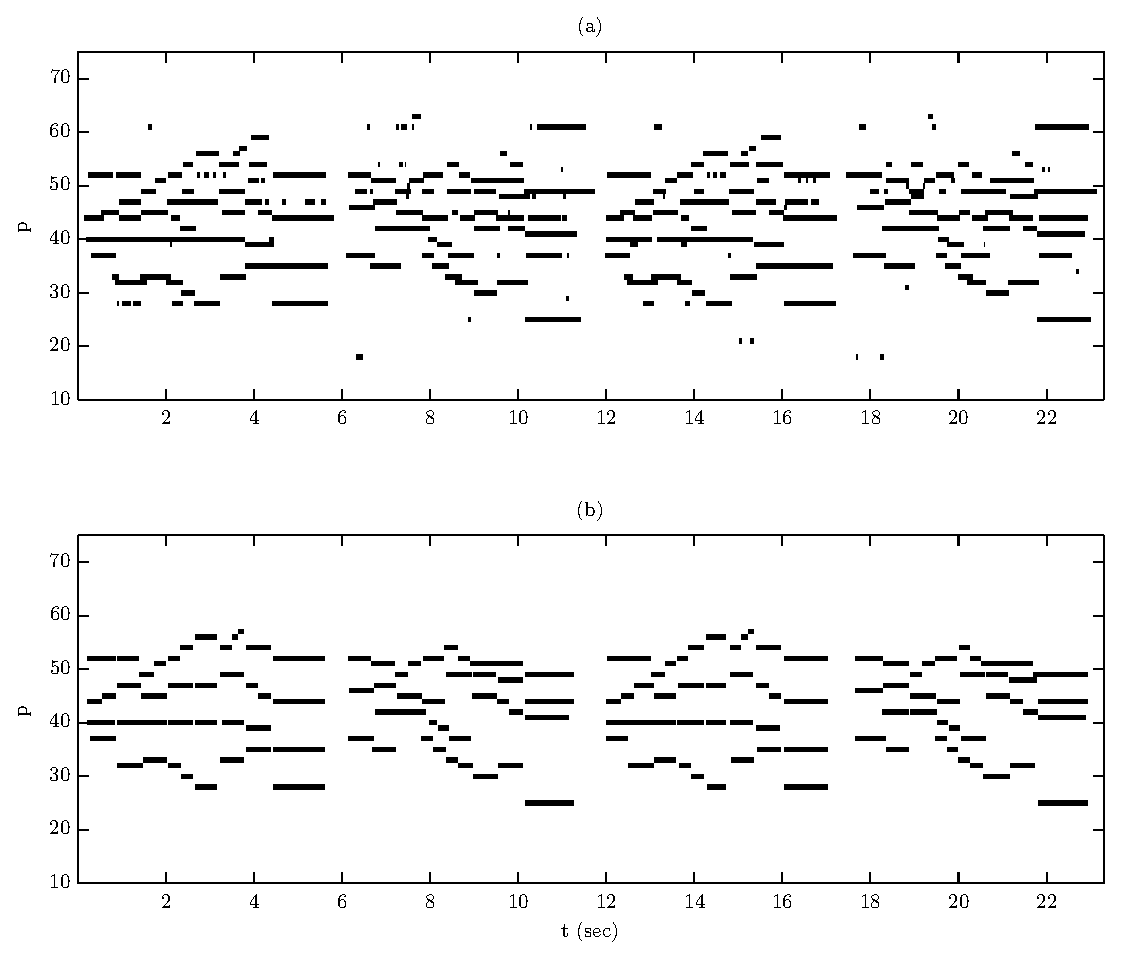
\includegraphics{figures/FigTranscription.eps}
 }
 \caption{Transcription example for recording ``Ach Lieben Christen'' from the Bach10 dataset. (a) The post-processed output of the transcription-predicton system using the 3rd configuration, with the NADE-HF. (b) The pitch ground truth of the recording.}
 \label{fig:Transcription}
\end{figure}

